\documentclass{article}




\usepackage{fullpage}
\usepackage{nopageno}
\usepackage{amsmath}
\usepackage{amsfonts}
\usepackage{graphicx}
\usepackage{framed}
\usepackage{algorithmic}
\usepackage{xcolor}

\definecolor{dark_red}{rgb}{0.5,0.0,0.0}
\definecolor{dark_green}{rgb}{0.0,0.5,0.0}
\definecolor{dark_blue}{rgb}{0.0,0.0,0.5}
\definecolor{blue}{rgb}{0.0,0.0,1.0}

\newcommand{\dr}[1]{\textcolor{dark_red}{#1}}
\newcommand{\dg}[1]{\textcolor{dark_green}{#1}}
\newcommand{\db}[1]{\textcolor{dark_blue}{#1}}
\newcommand{\blue}[1]{\textcolor{blue}{#1}}



\usepackage{fancyhdr}
%\setlength{\footheight}{15.2pt}
\pagestyle{fancy}
\fancyhead[C]{Wentworth Institute of Technology, MATH2025}
\fancyfoot[C]{Author: Shawn Eastwood}
\renewcommand{\headsep}{25pt}
\renewcommand{\headrulewidth}{1pt}
\renewcommand{\footrulewidth}{1pt}



\begin{document}

\section*{Single variable integrals}

Given a single variable function \(f(x)\), the definite integral of \(f(x)\) over the interval \([a, b]\) is defined by the following Riemann sum:

Let \(N\) denote a large integer. Partition the interval \([a, b]\) into a series of \(N\) intervals as depicted below:

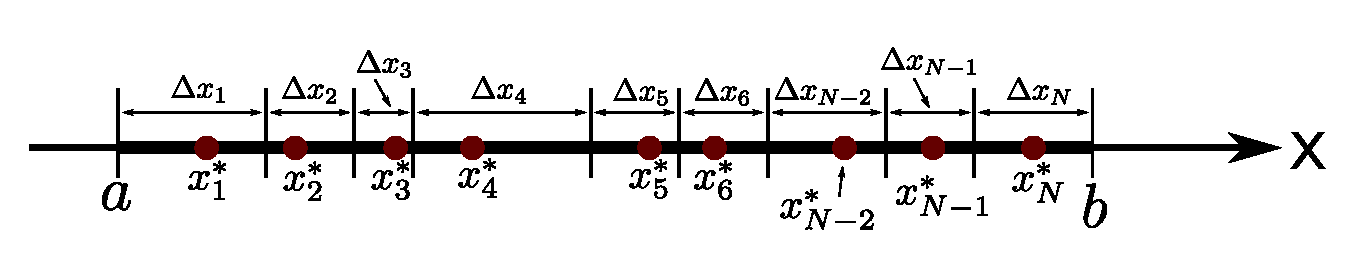
\includegraphics[width = \textwidth]{single_integral_riemann_sum}

For each \(i = 1, 2, ..., N\), the \(i^{\text{th}}\) interval has a length of \(\Delta x_i\) and contains the ``representative" point \(x_i^*\). The definite integral of \(f(x)\) over the interval \([a, b]\) is the limit:

\[\int_{x = a}^b f(x)dx = \lim_{N \rightarrow +\infty} \sum_{i=1}^N f(x_i^*)\Delta x_i\] 

The concept will now be generalized in order to integrate multivariable functions. 



\section*{Double integrals}

\begin{tabular}{cc}
\parbox{0.5\textwidth}{  
Given a function \(f(\mathbf{q})\) whose domain is a set of points in 2D space, the {\bf double integral} of \(f(\mathbf{q})\) over the 2D region \(R \subseteq \mathbb{R}^2\) is defined by the following Riemann sum: 

Let \(N\) denote a large integer. Partition the region \(R\) into a set of \(N\) tiny regions as depicted to the right. 

For each \(i = 1, 2, ..., N\), the \(i^{\text{th}}\) section has an area of \(\Delta A_i\) and contains the ``representative" point \(\mathbf{q}_i^*\). The double integral of \(f(\mathbf{q})\) over the region \(R\) is the limit:

\[\iint_{R} f(\mathbf{q})dA = \lim_{N \rightarrow +\infty} \sum_{i=1}^N f(\mathbf{q}_i^*)\Delta A_i\] 

} & \parbox{0.5\textwidth}{
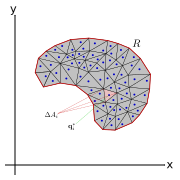
\includegraphics[width = 0.5\textwidth]{double_integral_riemann_sum}
}
\end{tabular}

If the integrand \(f(\mathbf{q})\) is \(1\), then the double integral evaluates to:
\[\iint_{R} dA = \lim_{N \rightarrow +\infty} \sum_{i=1}^N \Delta A_i = \text{area of \(R\)}\]
The area of a 2D region is the double integral of \(1\) over that region.


\section*{Double integrals using Cartesian coordinates}

~

\begin{tabular}{cc}  
\parbox{0.5\textwidth}{
2D regions can be quantified by first establishing bounds on the \(x\)-coordinate, and then establishing bounds on the \(y\)-coordinate that are functions of \(x\). This is referred to as a ``Type I" region. In the image on the right, the bounds on \(x\) are \(a\) and \(b\): \(a \leq x \leq b\). The bounds on \(y\) are functions of \(x\): \(h_L(x) \leq y \leq h_U(x)\). The region itself is:
\[R = \{(x,y) | a \leq x \leq b \;\&\; h_L(x) \leq y \leq h_U(x)\}\]
} & \parbox{0.5\textwidth}{
\includegraphics[width = 0.5\textwidth]{Cartesian_Regions_Type_I}
}
\end{tabular}

\begin{tabular}{cc}  
\parbox{0.5\textwidth}{
2D regions can also be quantified by first establishing bounds on the \(y\)-coordinate, and then establishing bounds on the \(x\)-coordinate that are functions of \(y\). This is referred to as a ``Type II" region, which essentially a Type I region with the roles of \(x\) and \(y\) reversed. In the image on the right, the bounds on \(y\) are \(a\) and \(b\): \(a \leq y \leq b\). The bounds on \(x\) are functions of \(y\): \(h_L(y) \leq x \leq h_U(y)\). The region itself is:
\[R = \{(x,y) | a \leq y \leq b \;\&\; h_L(y) \leq x \leq h_U(y)\}\]
} & \parbox{0.5\textwidth}{
\includegraphics[width = 0.5\textwidth]{Cartesian_Regions_Type_II}
}
\end{tabular}

\begin{tabular}{cc}
\parbox{0.5\textwidth}{
Not every region is a type I or a type II region. 
\begin{itemize}
\item To be a type I region, the range of \(x\) values must form a continuous interval \([a, b]\) with no gaps, and then fixing the value of \(x\), the range of \(y\) values must form a continuous interval \([h_L(x), h_U(x)]\) with no gaps. 
\item To be a type II region, the range of \(y\) values must form a continuous interval \([a, b]\) with no gaps, and then fixing the value of \(y\), the range of \(x\) values must form a continuous interval \([h_L(y), h_U(y)]\) with no gaps. 
\end{itemize}
In the image to the right, the lower left region is both a type I and a type II region. The lower right region is a type I but not a type II region. The upper left region is a type II but not a type I region. The upper right region is neither a type I or type II region.
} & \parbox{0.5\textwidth}{
\includegraphics[width = 0.5\textwidth]{Cartesian_Regions_Type_I_II}
}
\end{tabular}

The double integral \(\iint_R f(x,y)dA\) over the type I region:
\[R = \{(x,y) | a \leq x \leq b \;\&\; h_L(x) \leq y \leq h_U(x)\}\]
will now be evaluated using a series of two single variable integrals. To establish the single integral expression for \(\iint_R f(x,y)dA\), region \(R\) will be decomposed into a series of \(N\) vertical slivers where \(N\) is a large number, as depicted in the image below. For each \(i = 1, 2, ..., N\), the width of the \(i^{\text{th}}\) sliver is \(\Delta x_i\), and \(x_i^*\) is a ``representative" \(x\) value from the \(i^{\text{th}}\) sliver. Now for each vertical sliver, further partition the sliver into a series of \(M\) rectangles where \(M\) is a large number, as depicted in the image below. For each \(i = 1, 2, ..., N\) and for each \(j = 1, 2, ..., M\), the height of the \(j^{\text{th}}\) rectangle in the \(i^{\text{th}}\) sliver is \(\Delta y_{(i,j)}\), and \(y_{(i,j)}^*\) is a ``representative" \(y\) value from the \(j^{\text{th}}\) rectangle in the \(i^{\text{th}}\) sliver. The area of the \(j^{\text{th}}\) rectangle in the \(i^{\text{th}}\) sliver is \(\Delta A_{(i,j)} = \Delta x_i \Delta y_{(i,j)}\). 

\begin{center}
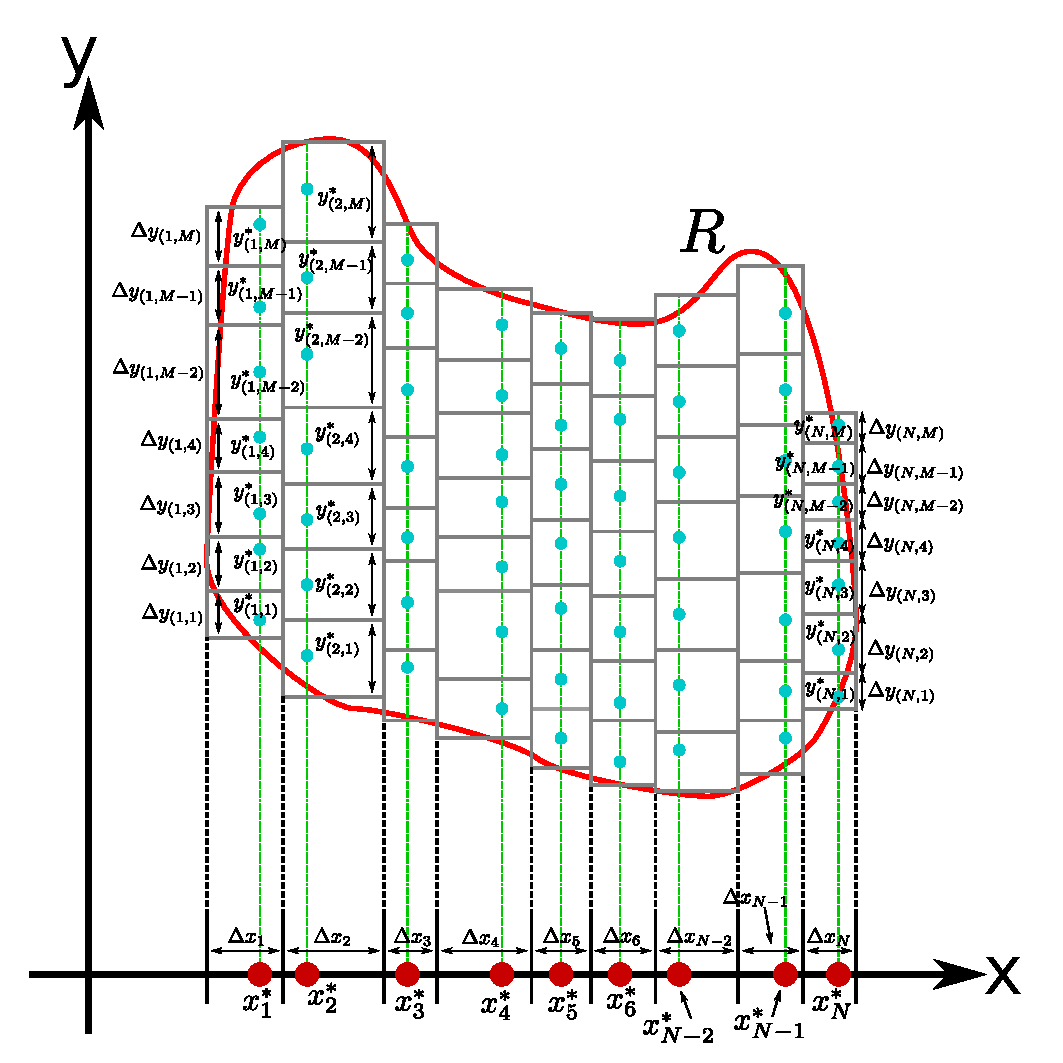
\includegraphics[width = \textwidth]{cartesian_type_1_riemann_sum}
\end{center}

Evaluating the Riemann sum gives:
\begin{align*}
\iint_R f(x,y)dA = & \lim_{N \rightarrow +\infty} \lim_{M \rightarrow +\infty} \sum_{i = 1}^N \sum_{j = 1}^M f(x_i^*,y_{(i,j)}^*) \Delta A_{(i,j)} 
= \lim_{N \rightarrow +\infty} \lim_{M \rightarrow +\infty} \sum_{i = 1}^N \sum_{j = 1}^M f(x_i^*,y_{(i,j)}^*) (\Delta x_i \Delta y_{(i,j)}) \\  
= & \lim_{N \rightarrow +\infty} \sum_{i = 1}^N \bigg(\lim_{M \rightarrow +\infty} \sum_{j = 1}^M f(x_i^*,y_{(i,j)}^*)\Delta y_{(i,j)}\bigg)\Delta x_i \\ 
= & \lim_{N \rightarrow +\infty} \sum_{i = 1}^N \bigg(\int_{y = h_L(x_i^*)}^{h_U(x_i^*)} f(x_i^*,y)dy\bigg)\Delta x_i  
= \int_{x = a}^b \bigg(\int_{y = h_L(x)}^{h_U(x)} f(x,y)dy\bigg)dx
\end{align*}

Therefore:
\[\iint_R f(x,y)dA = \int_{x = a}^b \bigg(\int_{y = h_L(x)}^{h_U(x)} f(x,y)dy\bigg)dx\]
This expression involving the repeated single variable integrals is often referred to as an ``{\bf iterated integral}" or a ``{\bf nested integral}".

For type II regions where the roles of \(x\) and \(y\) are reversed, if:
\[R = \{(x,y) | a \leq y \leq b \;\&\; h_L(y) \leq x \leq h_U(y)\}\]
then
\[\iint_R f(x,y)dA = \int_{y = a}^b \bigg(\int_{x = h_L(y)}^{h_U(y)} f(x,y)dx\bigg)dy\]


\subsection*{Reversing the order of integration}

Double integrals can be used to swap the order of integration for a nested integral. Let \(R\) have the type I and type II characterizations:
\[R = \{(x, y) | a \leq x \leq b \;\&\; h_L(x) \leq y \leq h_U(x)\} = \{(x, y) | c \leq y \leq d \;\&\; g_L(y) \leq x \leq g_U(y)\}\]
and let \(f(x,y)\) be an arbitrary integrand. The following nested integrals are now equivalent:
\[\int_{x = a}^b \left(\int_{y = h_L(x)}^{h_U(x)} f(x,y)dy\right)dx = \iint_R f(x,y)dA = \int_{y = c}^d \left(\int_{x = g_L(y)}^{g_U(y)} f(x,y)dx\right)dy\]



\pagebreak

%%%%%%%%%%%%%%%%%%%%%%%%%
\textbf{Example 1:}

\vspace{5mm}

\begin{tabular}{cc}
\parbox{0.5\textwidth}{
Consider the triangular region \(R\) to the right. This region can be characterized as both a type I and a type II region.    

For a type I characterization, the bounds on \(x\) are \(0\) and \(3\). The equation of the line that forms the hypotenuse of the triangle is: 
\begin{align*}
& y - 4 = \frac{0 - 4}{3 - 0}(x - 0) 
\iff y - 4 = -\frac{4}{3}x \\
& \iff y = 4 - \frac{4}{3}x
\end{align*}
The bounds on \(y\) as functions of \(x\) are \(0\) and \(4 - \frac{4}{3}x\). Therefore:
\[R = \left\{(x,y) \middle| 0 \leq x \leq 3 \;\&\; 0 \leq y \leq 4 - \frac{4}{3}x\right\}\]

For a type II characterization, the bounds on \(y\) are \(0\) and \(4\). The equation of the line that forms the hypotenuse of the triangle can be rearranged to get:
\[y = 4 - \frac{4}{3}x \iff -\frac{4}{3}x = y - 4 \iff x = 3 - \frac{3}{4}y\]
The bounds on \(x\) as functions of \(y\) are \(0\) and \(3 - \frac{3}{4}y\). Therefore:
\[R = \left\{(x,y) \middle| 0 \leq y \leq 4 \;\&\; 0 \leq x \leq 3 - \frac{3}{4}y\right\}\]

} & \parbox{0.5\textwidth}{
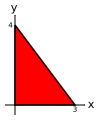
\includegraphics[width = 0.5\textwidth]{Example_1}
}
\end{tabular}
Now consider the arbitrary integrand \(f(x,y)\). The double integral \(\iint_R f(x,y)dA\) can be computed by using either the type I characterization: 
\[\iint_R f(x,y)dA = \int_{x = 0}^3 \left(\int_{y = 0}^{4 - \frac{4}{3}x} f(x,y)dy\right)dx\] 
or via the type II characterization: 
\[\iint_R f(x,y)dA = \int_{y = 0}^4 \left(\int_{x = 0}^{3 - \frac{3}{4}y} f(x,y)dx\right)dy\]

If the integrals in the nested integral need to be swapped, then:
\[\int_{x = 0}^3 \left(\int_{y = 0}^{4 - \frac{4}{3}x} f(x,y)dy\right)dx = \iint_R f(x,y)dA = \int_{y = 0}^4 \left(\int_{x = 0}^{3 - \frac{3}{4}y} f(x,y)dx\right)dy\]

Consider the specific integrand \(f(x, y) = x\). The double integral \(\iint_R x dA\) can now be evaluated via:

\begin{align*}
\iint_R x dA = & \int_{x = 0}^3 \left(\int_{y = 0}^{4 - \frac{4}{3}x} x dy\right)dx 
= \int_{x = 0}^3 \left(xy\Big|_{y = 0}^{4 - \frac{4}{3}x}\right)dx     
= \int_{x = 0}^3 \left(x\left(4 - \frac{4}{3}x\right) - 0\right)dx \\
= & \int_{x = 0}^3 \left(4x - \frac{4}{3}x^2\right)dx 
= \left.\left(2x^2 - \frac{4}{9}x^3\right)\right|_{x = 0}^3 
= (18 - 12) - 0 = 6
\end{align*}

or via:

\begin{align*}
\iint_R x dA = & \int_{y = 0}^4 \left(\int_{x = 0}^{3 - \frac{3}{4}y} x \cdot dx\right)dy 
= \int_{y = 0}^4 \left(\frac{1}{2}x^2\Big|_{x = 0}^{3 - \frac{3}{4}y}\right)dy  
= \int_{y = 0}^4 \left(\frac{1}{2}\left(3 - \frac{3}{4}y\right)^2 - 0\right)dy \\  
= & \int_{y = 0}^4 \left(\frac{9}{2} - \frac{9}{4}y + \frac{9}{32}y^2\right)dy 
= \left.\left(\frac{9}{2}y - \frac{9}{8}y^2 + \frac{3}{32}y^3\right)\right|_{y = 0}^4 
= (18 - 18 + 6) - 0 = 6
\end{align*}

Note that the final answer is the same either way.

Now consider the nested integral:
\[\int_{y = 0}^4 \left(\int_{x = 0}^{3 - \frac{3}{4}y} e^{4x - \frac{2}{3}x^2}dx\right)dy\] 
This nested integral is difficult to directly evaluate. By reversing the order of the variables, the solution becomes clear:
\begin{align*}
& \int_{y = 0}^4 \left(\int_{x = 0}^{3 - \frac{3}{4}y} e^{4x - \frac{2}{3}x^2}dx\right)dy  
= \iint_R e^{4x - \frac{2}{3}x^2}dA 
= \int_{x = 0}^3 \left(\int_{y = 0}^{4 - \frac{4}{3}x} e^{4x - \frac{2}{3}x^2}dy\right)dx \\ 
& = \int_{x = 0}^3 \left(y \cdot e^{4x - \frac{2}{3}x^2}\Big|_{y = 0}^{4 - \frac{4}{3}x}\right)dx
= \int_{x = 0}^3 \left((4 - \frac{4}{3}x)e^{4x - \frac{2}{3}x^2}\right)dx 
= e^{4x - \frac{2}{3}x^2}\Big|_{x = 0}^3 \\
& = e^{12 - 6} - e^0
= e^6 - 1
\end{align*}



\pagebreak

%%%%%%%%%%%%%%%%%%%%%%%%%
\textbf{Example 2:}  

\vspace{5mm}

\begin{tabular}{cc}
\parbox{0.5\textwidth}{
Consider the parabolic region on the right. This region can be characterized as both a type I and a type II region.    

For a type I characterization, the bounds on \(x\) are \(-4\) and \(0\). The equation of the parabola is: 
\[y = 5 - \frac{5}{16}x^2\]
The bounds on \(y\) as functions of \(x\) are \(0\) and \(5 - \frac{5}{16}x^2\). Therefore:
\[R = \left\{(x,y) \middle| -4 \leq x \leq 0 \;\&\; 0 \leq y \leq 5 - \frac{5}{16}x^2\right\}\]

For a type II characterization, the bounds on \(y\) are \(0\) and \(5\). The equation of the parabola can be rearranged to get: 
\begin{align*}
& y = 5 - \frac{5}{16}x^2 \iff -\frac{5}{16}x^2 = y - 5 \\
& \iff x^2 = 16 - \frac{16}{5}y \iff x = \pm 4\sqrt{1 - \frac{y}{5}}
\end{align*}
The upper bound on \(x\) is \(0\), while the lower bound on \(x\) as a function of \(y\) must be \(\leq 0\), so this lower bound is \(-4\sqrt{1 - \frac{y}{5}}\). Therefore:
\[R = \left\{(x,y) \middle| 0 \leq y \leq 5 \;\&\; -4\sqrt{1 - \frac{y}{5}} \leq x \leq 0\right\}\]

} & \parbox{0.5\textwidth}{
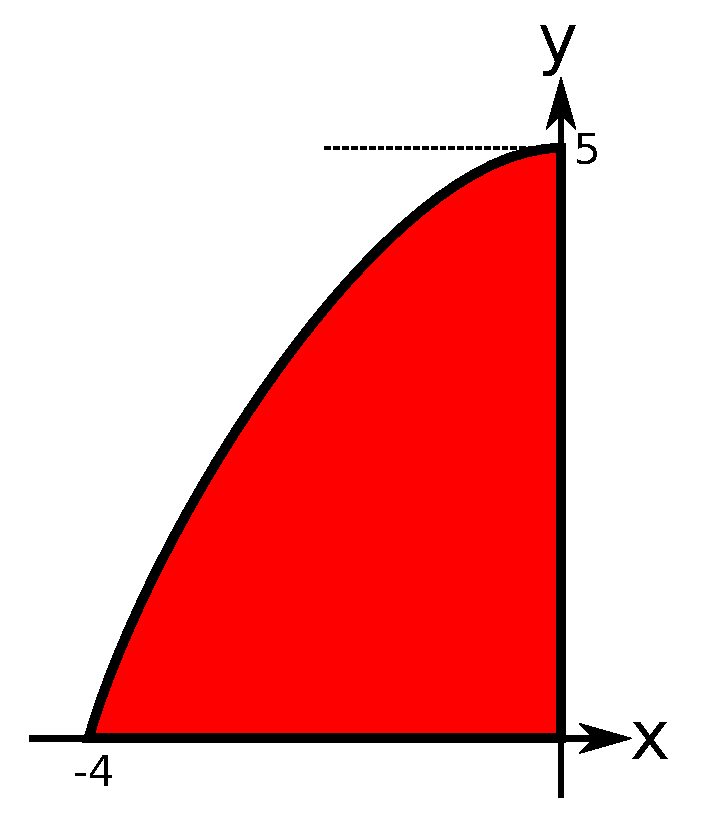
\includegraphics[width = 0.5\textwidth]{Example_2}
}
\end{tabular}
Now consider the arbitrary integrand \(f(x,y)\). The double integral \(\iint_R f(x,y)dA\) can be computed by using either the type I characterization: 
\[\iint_R f(x,y)dA = \int_{x = -4}^0 \left(\int_{y = 0}^{5 - \frac{5}{16}x^2} f(x,y)dy\right)dx\] 
or via the type II characterization: 
\[\iint_R f(x,y)dA = \int_{y = 0}^5 \left(\int_{x = -4\sqrt{1 - \frac{y}{5}}}^{0} f(x,y)dx\right)dy\]

If the integrals in the nested integral need to be swapped, then:
\[\int_{x = -4}^0 \left(\int_{y = 0}^{5 - \frac{5}{16}x^2} f(x,y)dy\right)dx = \int_{y = 0}^5 \left(\int_{x = -4\sqrt{1 - \frac{y}{5}}}^{0} f(x,y)dx\right)dy\]

Consider the specific integrand \(f(x, y) = \frac{1}{\sqrt{5-y}}\). The double integral \(\iint_R \frac{1}{\sqrt{5-y}} dA\) can now be evaluated via:

\begin{align*}
\iint_R \frac{1}{\sqrt{5-y}} dA = & \int_{x = -4}^0 \left(\int_{y = 0}^{5 - \frac{5}{16}x^2} \frac{1}{\sqrt{5-y}}dy\right)dx 
= \int_{x = -4}^0 \left(-2\sqrt{5-y}\Big|_{y = 0}^{5 - \frac{5}{16}x^2} \right)dx \\
= & \int_{x = -4}^0 \left(-2\sqrt{\frac{5}{16}x^2} - (-2\sqrt{5}) \right)dx 
= \int_{x = -4}^0 \left(-\frac{\sqrt{5}}{2}|x| + 2\sqrt{5} \right)dx \\  
= & \int_{x = -4}^0 \left(\frac{\sqrt{5}}{2}x + 2\sqrt{5} \right)dx 
= \left.\left(\frac{\sqrt{5}}{4}x^2 + (2\sqrt{5})x \right)\right|_{x = -4}^0 \\
= & 0 - \left(4\sqrt{5} - 8\sqrt{5}\right) 
= 4\sqrt{5}
\end{align*}

or via:

\begin{align*} 
\iint_R \frac{1}{\sqrt{5-y}} dA = & \int_{y = 0}^5 \left(\int_{x = -4\sqrt{1 - \frac{y}{5}}}^{0} \frac{1}{\sqrt{5-y}}dx\right)dy 
= \int_{y = 0}^5 \left(\frac{x}{\sqrt{5-y}}\bigg|_{x = -4\sqrt{1 - \frac{y}{5}}}^{0}\right)dy \\ 
= & \int_{y = 0}^5 \left(0 - \frac{-4\sqrt{1 - \frac{y}{5}}}{\sqrt{5-y}}\right)dy 
= \int_{y = 0}^5 \frac{(4/\sqrt{5})\sqrt{5 - y}}{\sqrt{5-y}}dy 
= \int_{y = 0}^5 \frac{4}{\sqrt{5}}dy \\
= & \left.\frac{4y}{\sqrt{5}}\right|_{y = 0}^5   
= 4\sqrt{5}
\end{align*} 

Note that the final answer is the same either way.

Now consider the nested integral: 
\[\int_{x = -4}^0 \left(\int_{y = 0}^{5 - \frac{5}{16}x^2} \cos((5 - y)^{3/2})dy\right)dx\]
This nested integral is difficult to directly evaluate. By reversing the order of the variables, the solution becomes clear:
\begin{align*} 
& \int_{x = -4}^0 \left(\int_{y = 0}^{5 - \frac{5}{16}x^2} \cos((5 - y)^{3/2})dy\right)dx 
= \iint_R \cos((5 - y)^{3/2})dA \\
& = \int_{y = 0}^5 \left(\int_{x = -4\sqrt{1 - \frac{y}{5}}}^{0} \cos((5 - y)^{3/2})dx\right)dy 
= \int_{y = 0}^5 \left(x\cos((5 - y)^{3/2})\Big|_{x = -4\sqrt{1 - \frac{y}{5}}}^{0}\right)dy \\ 
& = \int_{y = 0}^5 \frac{4}{\sqrt{5}} \cdot \sqrt{5 - y} \cdot \cos((5 - y)^{3/2}) dy  
= \int_{y = 0}^5 \frac{-8}{3\sqrt{5}} \cdot \cos((5 - y)^{3/2}) \cdot \frac{3}{2}(5 - y)^{1/2} \cdot (-1) dy \\
& = \frac{-8}{3\sqrt{5}} \cdot \sin((5 - y)^{3/2})\bigg|_{y = 0}^5 
= 0 - \frac{-8}{3\sqrt{5}} \cdot \sin(5^{3/2})  
= \frac{8}{3\sqrt{5}} \cdot \sin(5^{3/2})
\end{align*}



\pagebreak

%%%%%%%%%%%%%%%%%%%%%%%%%
\textbf{Example 3:}  

\vspace{5mm}

\begin{tabular}{cc}
\parbox{0.5\textwidth}{
Consider the parabolic region on the right. This region can be characterized as both a type I and a type II region.    

For a type I characterization, the bounds on \(x\) are \(-2\) and \(0\). The equation of the parabola is:
\[y = -(x + 2)^2\]
The bounds on \(y\) as functions of \(x\) are \(-(x + 2)^2\) and \(0\). Therefore:
\[R = \left\{(x,y) \middle| -2 \leq x \leq 0 \;\&\; -(x + 2)^2 \leq y \leq 0\right\}\]

For a type II characterization, the bounds on \(y\) are \(-4\) and \(0\). The equation of the parabola can be rearranged to get: 
\begin{align*}
& y = -(x + 2)^2 \iff (x + 2)^2 = -y \\
& \iff x + 2 = \pm\sqrt{-y} \iff x = -2 \pm\sqrt{-y}
\end{align*}
The upper bound on \(x\) is \(0\), while the lower bound on \(x\) as a function of \(y\) must be \(\geq -2\) , so this lower bound is \(-2 + \sqrt{-y}\). Therefore:
\[R = \left\{(x,y) \middle| -4 \leq y \leq 0 \;\&\; -2 + \sqrt{-y} \leq x \leq 0\right\}\]

} & \parbox{0.5\textwidth}{

\includegraphics[width = 0.35\textwidth]{Example_3}
}
\end{tabular}
Now consider the arbitrary integrand \(f(x,y)\). The double integral \(\iint_R f(x,y)dA\) can be computed by using either the type I characterization: 
\[\iint_R f(x,y)dA = \int_{x = -2}^0 \left(\int_{y = -(x + 2)^2}^0 f(x,y)dy\right)dx\] 
or via the type II characterization: 
\[\iint_R f(x,y)dA = \int_{y = -4}^0 \left(\int_{x = -2 + \sqrt{-y}}^{0} f(x,y)dx\right)dy\]

If the integrals in the nested integral need to be swapped, then:
\[\int_{x = -2}^0 \left(\int_{y = -(x + 2)^2}^0 f(x,y)dy\right)dx = \int_{y = -4}^0 \left(\int_{x = -2 + \sqrt{-y}}^{0} f(x,y)dx\right)dy\]

Consider the specific integrand \(f(x, y) = x + 2\). The double integral \(\iint_R (x + 2)dA\) can now be evaluated via:

\begin{align*}
\iint_R (x + 2)dA = & \int_{x = -2}^0 \left(\int_{y = -(x + 2)^2}^{0} (x + 2)dy\right)dx 
= \int_{x = -2}^0 \left((x + 2)y\Big|_{y = -(x + 2)^2}^{0} \right)dx \\
= & \int_{x = -2}^0 \left(0 - (-(x + 2)^3) \right)dx 
= \int_{x = -2}^0 (x + 2)^3 dx \\  
= & \left.\frac{1}{4}(x + 2)^4\right|_{x = -2}^0 
= \frac{1}{4} \cdot 2^4 - 0 
= 4
\end{align*}

or via:

\begin{align*} 
\iint_R (x + 2)dA = & \int_{y = -4}^0 \left(\int_{x = -2 + \sqrt{-y}}^{0} (x + 2)dx\right)dy 
= \int_{y = -4}^0 \left((\frac{1}{2}x^2 + 2x)\bigg|_{x = -2 + \sqrt{-y}}^{0}\right)dy \\ 
= & \int_{y = -4}^0 \left(0 - (\frac{1}{2}(4 - 4\sqrt{-y} - y) + 2(-2 + \sqrt{-y}))\right)dy \\
= & \int_{y = -4}^0 \left(-((2 - 2\sqrt{-y} - \frac{1}{2}y) + (-4 + 2\sqrt{-y}))\right)dy 
= \int_{y = -4}^0 \left(2 + \frac{1}{2}y\right)dy \\
= & \left.(2y + \frac{1}{4}y^2)\right|_{y = -4}^0   
= 0 - (-8 + 4)
= 4
\end{align*} 

Note that the final answer is the same either way.

Now consider the specific integrand \(f(x, y) = y\). The double integral \(\iint_R y dA\) can now be evaluated via:

\begin{align*}
\iint_R y dA = & \int_{x = -2}^0 \left(\int_{y = -(x + 2)^2}^{0} y dy\right)dx 
= \int_{x = -2}^0 \left(\frac{1}{2}y^2\Big|_{y = -(x + 2)^2}^{0} \right)dx \\
= & \int_{x = -2}^0 \left(0 - \frac{1}{2}(x + 2)^4 \right)dx 
= \int_{x = -2}^0 -\frac{1}{2}(x + 2)^4 dx \\  
= & \left.-\frac{1}{10}(x + 2)^5\right|_{x = -2}^0 
= -\frac{1}{10} \cdot 2^5 - 0 
= -\frac{16}{5}
\end{align*}

or via:

\begin{align*} 
\iint_R y dA = & \int_{y = -4}^0 \left(\int_{x = -2 + \sqrt{-y}}^{0} y dx\right)dy 
= \int_{y = -4}^0 \left(xy\bigg|_{x = -2 + \sqrt{-y}}^{0}\right)dy \\ 
= & \int_{y = -4}^0 \left(0 - (-2y + y\sqrt{-y})\right)dy 
= \int_{y = -4}^0 \left(2y + (-y)^{3/2}\right)dy 
= \left(y^2 - \frac{2}{5}(-y)^{5/2}\right)\bigg|_{y = -4}^0 \\
= & 0 - (16 - \frac{2}{5} \cdot 4^{5/2})   
= -(16 - \frac{64}{5})
= -\frac{16}{5}
\end{align*} 

Note that the final answer is the same either way.




\pagebreak

%%%%%%%%%%%%%%%%%%%%%%%%%
\textbf{Example 4:}  

\vspace{5mm}

\begin{tabular}{cc}
\parbox{0.5\textwidth}{
Consider the quarter circular region on the right. This region can be characterized as both a type I and a type II region.    

For a type I characterization, the bounds on \(x\) are \(-3\) and \(0\). The lower bound on \(y\) is \(0\). The upper bound on \(y\) as a function \(x\) is the circle with a radius of \(3\). The equation of the circular arc is: 
\begin{align*}
& (x + 3)^2 + y^2 = 9 
\iff y^2 = 9 - (x + 3)^2 \\
& \iff y = \pm\sqrt{9 - (x + 3)^2}
\end{align*}
The upper bound on \(y\) is positive, and is \(\sqrt{9 - (x + 3)^2}\). Therefore:
\[R = \left\{(x,y) \middle| -3 \leq x \leq 0 \;\&\; 0 \leq y \leq \sqrt{9 - (x + 3)^2}\right\}\]

For a type II characterization, the bounds on \(y\) are \(0\) and \(3\). The equation of the circular arc can be rearranged to get: 
\begin{align*}
& (x + 3)^2 + y^2 = 9 
\iff (x + 3)^2 = 9 - y^2 \\
& \iff x + 3 = \pm\sqrt{9 - y^2} 
\iff x = -3 \pm \sqrt{9 - y^2} 
\end{align*}
The lower bound on \(x\) is \(-3\), while the upper bound on \(x\) as a function of \(y\) must be \(\geq -3\), so this upper bound is \(-3 + \sqrt{9 - y^2}\). Therefore:
\[R = \left\{(x,y) \middle| 0 \leq y \leq 3 \;\&\; -3 \leq x \leq -3 + \sqrt{9 - y^2}\right\}\]

} & \parbox{0.5\textwidth}{
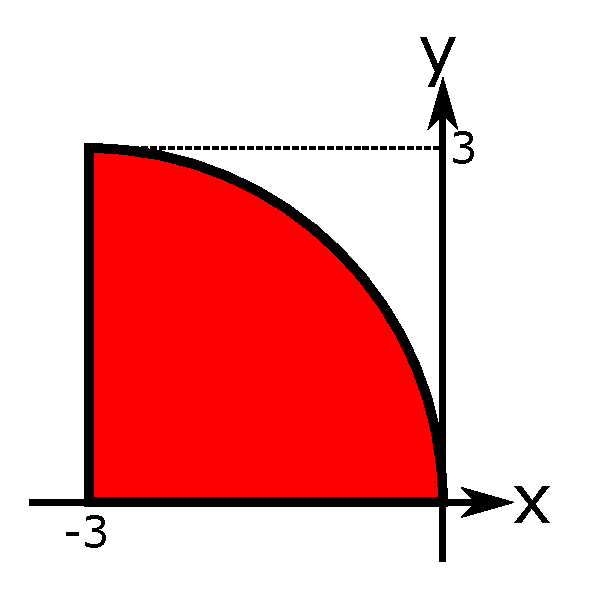
\includegraphics[width = 0.5\textwidth]{Example_4}
}
\end{tabular}
Now consider the arbitrary integrand \(f(x,y)\). The double integral \(\iint_R f(x,y)dA\) can be computed by using either the type I characterization: 
\[\iint_R f(x,y)dA = \int_{x = -3}^0 \left(\int_{y = 0}^{\sqrt{9 - (x + 3)^2}} f(x,y)dy\right)dx\] 
or via the type II characterization: 
\[\iint_R f(x,y)dA = \int_{y = 0}^3 \left(\int_{x = -3}^{-3 + \sqrt{9 - y^2}} f(x,y)dx\right)dy\]

If the integrals in the nested integral need to be swapped, then:
\[\int_{x = -3}^0 \left(\int_{y = 0}^{\sqrt{9 - (x + 3)^2}} f(x,y)dy\right)dx = \int_{y = 0}^3 \left(\int_{x = -3}^{-3 + \sqrt{9 - y^2}} f(x,y)dx\right)dy\]



\pagebreak

%%%%%%%%%%%%%%%%%%%%%%%%%
\textbf{Example 5:}

\vspace{5mm}

\begin{tabular}{cc}
\parbox{0.5\textwidth}{
Consider the region on the right. This region is bounded from below by the parabola \(y = x^2\) and from above by the line \(y = 3x\). This region can be characterized as both a type I and a type II region.    

For a type I characterization, the bounds on \(x\) are \(0\) and \(3\). The bounds on \(y\) as functions of \(x\) are \(x^2\) and \(3x\). Therefore:
\[R = \left\{(x,y) \middle| 0 \leq x \leq 3 \;\&\; x^2 \leq y \leq 3x\right\}\]

For a type II characterization, the bounds on \(y\) are \(0\) and \(9\). The equation of the line can be rearranged to get the lower bound on \(x\): 
\[y = 3x \iff x = \frac{y}{3}\]
The equation of the parabola can be rearranged to get the upper bound on \(x\):
\[y = x^2 \iff x = \pm \sqrt{y}\]
The upper bound of \(x\) must be \(\geq 0\), so the upper bound is \(\sqrt{y}\). Therefore:
\[R = \left\{(x,y) \middle| 0 \leq y \leq 9 \;\&\; \frac{y}{3} \leq x \leq \sqrt{y}\right\}\]

} & \parbox{0.5\textwidth}{

\includegraphics[width = 0.5\textwidth]{Example_5}
}
\end{tabular}
Now consider the arbitrary integrand \(f(x,y)\). The double integral \(\iint_R f(x,y)dA\) can be computed by using either the type I characterization: 
\[\iint_R f(x,y)dA = \int_{x = 0}^3 \left(\int_{y = x^2}^{3x} f(x,y)dy\right)dx\] 
or via the type II characterization: 
\[\iint_R f(x,y)dA = \int_{y = 0}^9 \left(\int_{x = y/3}^{\sqrt{y}} f(x,y)dx\right)dy\]

If the integrals in the nested integral need to be swapped, then: 
\[\int_{x = 0}^3 \left(\int_{y = x^2}^{3x} f(x,y)dy\right)dx = \int_{y = 0}^9 \left(\int_{x = y/3}^{\sqrt{y}} f(x,y)dx\right)dy\]



\pagebreak

\section*{Rectangular regions}

\begin{tabular}{cc}
\parbox{0.5\textwidth}{
A rectangular region \(R\) is a region where the bounds on \(x\) and \(y\) are entirely independent of each other. The bounds are constant, and fixing \(x\) to different values does not change the bounds on \(y\), and vice versa.
\[R = [a, b] \times [c, d] = \{(x, y) | a \leq x \leq b \;\&\; c \leq y \leq d\}\]
A rectangular region is both a type I and a type II region. Moreover, the order of integration in a nested integral over a rectangular region can be reversed by simply swapping the integral signs without any further considerations:
\[\int_{x = a}^b \left(\int_{y = c}^d f(x,y)dy\right)dx = \int_{y = c}^d \left(\int_{x = a}^b f(x,y)dx\right)dy\]
} & \parbox{0.5\textwidth}{
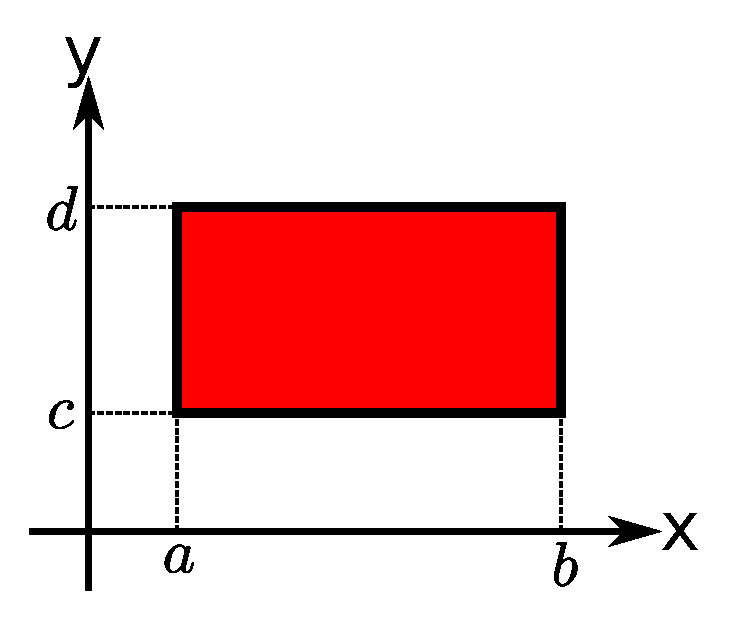
\includegraphics[width = 0.5\textwidth]{rectangular_regions}
}
\end{tabular}


Given two single variable functions \(g(x)\) and \(h(x)\), and the definite integrals \(\int_{x = a}^b g(x)dx\) and \(\int_{x = c}^d h(x)dx\), then the product of these definite integrals is a double integral of the product \(g(x)h(y)\) over the rectangular region \(R = [a, b] \times [c, d] = \{(x, y) | a \leq x \leq b \;\&\; c \leq y \leq d\}\): 

\begin{align*}
& \left(\int_{x = a}^b g(x)dx\right)\left(\int_{x = c}^d h(x)dx\right) \\
& = \left(\int_{x = a}^b g(x)dx\right)\left(\int_{y = c}^d h(y)dy\right) & \begin{array}{c} \text{Replace the local placeholder variable of \(x\) in the second integral} \\ \text{with the distinct symbol \(y\).}\end{array} \\
& = \int_{x = a}^b g(x)\left(\int_{y = c}^d h(y)dy\right)dx & \begin{array}{c} \text{\(\int_{y = c}^d h(y)dy\) is constant with respect to \(x\).} \end{array} \\ 
& = \int_{x = a}^b \left(\int_{y = c}^d g(x)h(y)dy\right)dx & \begin{array}{c} \text{\(g(x)\) is constant with respect to \(y\).} \end{array} \\ 
& = \iint_R g(x)h(y) dA
\end{align*}
Therefore:
\[\left(\int_{x = a}^b g(x)dx\right)\left(\int_{x = c}^d h(x)dx\right) = \iint_R g(x)h(y) dA\]
 

\textbf{Examples:}

\begin{itemize}
\item Consider the rectangle \(R = \{(x, y) | -2 \leq x \leq 1 \;\&\; -1 \leq y \leq 1\}\) and the function \(f(x,y) = xy + 3x + 2y + 6\). 

\(f(x,y)\) can be factored to give \(f(x,y) = (x + 2)(y + 3)\) so the double integral of \(f(x,y)\) over the rectangle \(R\) is:

\begin{align*}
& \iint_R (x + 2)(y + 3)dA = \left(\int_{x = -2}^1 (x + 2)dx\right)\left(\int_{y = -1}^1 (y + 3)dy\right)  
= (\frac{1}{2}x^2 + 2x)\bigg|_{x = -2}^1 \cdot (\frac{1}{2}y^2 + 3y)\bigg|_{y = -1}^1 \\
& = ((\frac{1}{2} + 2) - (2 - 4)) \cdot ((\frac{1}{2} + 3) - (\frac{1}{2} - 3)) 
= (\frac{5}{2} + 2) \cdot (\frac{7}{2} + \frac{5}{2}) 
= \frac{9}{2} \cdot 6 
= 27
\end{align*}
 
\end{itemize}


\end{document}














